\documentclass[12pt]{article}
\usepackage[english]{babel}

% Set page size and margins
% Replace `letterpaper' with`a4paper' for UK/EU standard size
\usepackage[letterpaper,top=2cm,bottom=2cm,left=3cm,right=3cm,marginparwidth=1.75cm]{geometry}

% to typeset URLs, URIs, and DOIs
\usepackage[colorlinks=true, allcolors=blue]{hyperref}
\usepackage{url}
\usepackage{graphicx}
\usepackage[english]{babel}

% Bibliography
\usepackage[style=apa, backend=biber, natbib]{biblatex}
\addbibresource{References.bib}
%\usepackage{natbib}

% useful packages
\usepackage{amsmath,amsfonts,amssymb,amsthm,mathtools,mathrsfs}
\usepackage{csquotes}
\usepackage{caption,subcaption}
\captionsetup{compatibility=false}
\usepackage{xcolor}
\usepackage{soul}
\usepackage{float}
\def\UrlFont{\rmfamily}

\renewcommand \thesection{\Roman{section}}
\renewcommand \thesubsection{\arabic{section}.\arabic{subsection}}


\begin{document}

\title{Machine Learning for NFT Price Predictions}


\author{Mingxuan He\thanks{mingxuanh@uchicago.edu, Chicago, IL, United States of America}}
\date{\today}


\maketitle 


\begin{abstract}
In this proposal, I outline the motivation, data, methods, and preliminary results of my project. The goal of this project is to predict the price of NFTs using classical machine learning and deep learning methods. Training and testing data include transactions data from the Ethereum blockchain via Dune Analytics, and NFT collection data from OpenSea, the largest NFT marketplace. The results will be presented in a paper and a presentation. The code will be written in Python utilizing packages including scikit-learn and tensorflow.\\

\textbf{Keywords:} NFTs, machine learning, onchain data, predictive modeling

\end{abstract} 

%\tableofcontents


\section{Introduction}
\label{sec: introduction}
A non-fungible token (NFT) is a digital asset stored on a blockchain. The uniqueness of each NFT asset is verifiable through the unique identification assigned by the blockchain on which they exist.
NFTs can represent photos, videos, audio, and other types of digital files. NFTs are most commonly bought and sold with cryptocurrencies via digital marketplaces, with the Ethereum blockchain being the most popular market.

Recently, picture NFTs have emerged as a popular investment vehicle. For example, the NFT of a digital artwork by Beeple was sold for \$69 million in March 2021. The NFT market has grown rapidly since 2019, with the total trading volume exceeding \$12 billion in Q1 2022 alone.

Similar to their fungible counterpart (cryptocurrencies), a picture NFT can vary from a few dollars to millions of dollars. The price of a picture NFT is determined by a variety of factors, most notably the possession of ``rare traits". However, similar to the traditional arts market, most NFT prices are also heavily dependent on market taste and sentiment, such as the current popularity of the collection and/or the artist.

In this paper, I apply machine learning methods to predict the price of picture NFTs. Specifically, I train models on market prices and rarity data obtained from the Ethereum blockchain. The goal is to estalish a model framework that provides accurate estimates of NFT prices. Such a model has various applications, including but not limited to onchain trading and bidding contracts, risk management for crypto portfolios, and fair valuation of staked/collateralized NFTs for decentralized finance (DeFi) applications. In addition, the model can be used to price large batches of NFTs quickly, which is useful for AI-generated NFTs.

The rest of this paper is structured as follows. Section \ref{sec: lit_review} discusses the existing literature on this topic and the novelty of this paper. Section \ref{sec: data} provides an overview of the data used in this project. Section \ref{sec: method} outlines the general methodology and the machine learning models used in training. Section \ref{sec: results} presents the results. Section \ref{sec: conclusion} draws conclusions.


\section{Literature Review}
\label{sec: lit_review}
% market analysis
The fast-growing market of NFTs has attracted interest from various academic disciplines. In the economics and finance literature, various authors have discussed the price dynamics of the NFT market. A comprehensive work by \citet{nadini2021mapping} mapped out important statistical features of NFT markets, revealing that mean prices, sales per asset, sales per collection all follow power-law distributions. \citet{ante2022non} found that NFT sales are triggered by price shocks in Bitcoin (BTC) and active NFT wallets are reduced by price shocks in  Ether (ETH). Similarly, \citet{dowling2022non} found co-movement between cryptocurrencies and NFTs through wavelet coherence analysis. On the buyer side, \citet{kong2021alternative} that well-connected and experienced investors generally pay lower prices for NFTs. These results support the general belief that the NFT market is not fully efficient, and there is room for improvement in pricing NFTs. 

% rarity
The literature agrees on that rarity is one of, if not the most important factors in determining the price of NFTs. Using data from the CryptoPunks collection, \citet{kong2021alternative} built a hedonic regression model and highlighted rarity as a key determinant of price premium in the cross-section. \citet{mekacher2022heterogeneous} used a custom-built rarity score and showed that rarer NFTs sell for higher prices, are traded less frequently, guarantee higher returns, and are less risky. Taking a network clustering approach, \citet{nadini2021mapping} extracted vector representations of the visual features of NFTs and analyzed their cosine distance network using the pre-trained convolutional neural network AlexNet. These results inspired the inclusion of trait features and the OpenRarity rarity rank as a key set of features in my model.

% ML
In the applied machine learning literature, there have been notable attempts to apply regression models and neural networks to predict the price of NFTs. \citet{nadini2021mapping} used a linear regression model with network features such as the buyer's and seller's degree and PageRank centrality, principal components of the NFT's visual features, as well as market data such as the past median price of primary and secondary sales.

The literature also identified other features such as search trends \citep{jain2022nft,kaneko2021time}, social media influence e.g. Twitter \citep{kapoor2022tweetboost}.


\section{Background \& Data}
\label{sec: data}

\subsection{Institutional background}
The NFT market is an emerging market with unique aspects. In this section, I provide a brief overview of the background of NFT markets, including relevant terminology.

\begin{itemize}

    \item \textbf{NFT Marketplaces:} NFT Marketplaces are platforms built with automated blockchain contracts (known as ``smart contracts'') to facilitate transactions using cryptocurrencies. Most popular marketplaces include OpenSea, Blur, Rarible, SuperRare, etc. 

    \item \textbf{NFT Collections:} Many NFTs are created in collections, in which all NFTs share a common theme. For example, the CryptoPunks collection consists of 10,000 unique pictures of pixelated faces. 

    \item \textbf{Traits:} Each NFT in the collection has a unique combination of traits, including color, background, face/expression, and accessories. The traits typically differ by rarity. For example, there are more than 2,000 CryptoPunks with the trait ``Earring", but only 44 with the trait ``Beanie".
    
    \item \textbf{Rarity Score \& Rarity Rank: } The current industry standard for calculating the rarity of an NFT within a collection is the OpenRarity Standard \footnote{\url{https://www.openrarity.dev/}}, where the rarity of an NFT is evaluated on the rarity of its traits. The calculations for this metric is outlined in Appendix \ref{app: rarity}. By comparing the rarity score of all NFTs in a collection, we can rank the rarity of each NFT, with 1 being the rarest.
\end{itemize}

\subsection{Data sources}
I obtained data from two sources: Dune Analytics and OpenSea.

\subsubsection{Dune Analytics}
Dune Analytics is a platform for querying public databases from the Ethereum blockchain. For each collection, I query the NFT trades database and gather information on all NFT transactions from issuance to Sep 30, 2023.

\subsubsection{OpenSea}
OpenSea is the largest NFT marketplace focusing on NFTs based on Ethereum and Ethereum's Layer-2 ecosystem. The data from OpenSea's public API include data on NFT collections. In particular, I extracted data on the traits and rarity of each unique NFT in the collections. The set of available traits varies by collection, but generally include color, background, face/expression, and accessories.

\subsection{Exploratory analysis}
% TODO: summary stats with sample size
\begin{figure}[H]
    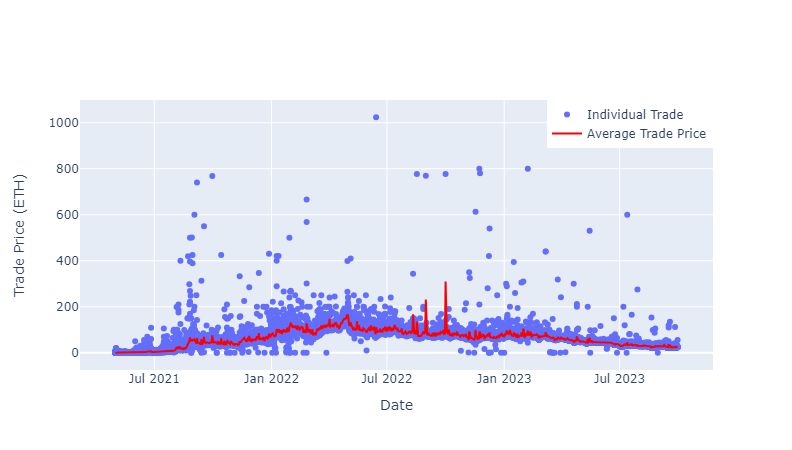
\includegraphics[width=\textwidth]{../figures/price_date.png}
    \caption{Trade Price by Date}
\end{figure}

\begin{figure}[H]
    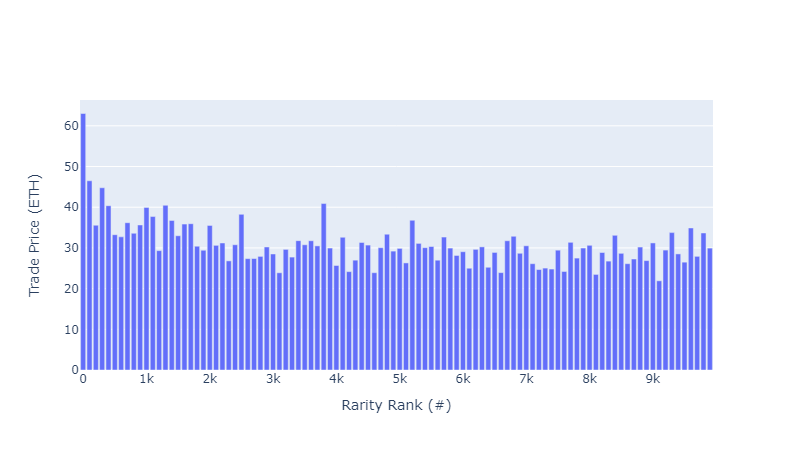
\includegraphics[width=\textwidth]{../figures/price_rarity.png}
    \caption{Trade Price by Rarity Rank}
\end{figure}


\section{Methodology}
\label{sec: method}
For benchmarking, I will use an OLS model. For the main model, I will use a neural network with a fully connected layer. I will also explore other deep learning methods, including convolutional neural networks (CNNs) and recurrent neural networks (RNNs). This is currently work in progress.


\section{Results}
\label{sec: results}


\section{Conclusion}
\label{sec: conclusion}


% \section*{Acknowledgements}
% \label{sec: acknowledgements}


\newpage
\printbibliography

\newpage
\appendix

\section{Rarity Score and Rarity Rank}
\label{app: rarity}
I use OpenSea's OpenRarity standard to calculate the rarity of each NFT within its collection. The rarity score is defined as follows:\\
For an NFT $x$ with traits $i\dots n$, its rarity score is
\[R(x) = \frac{I(x)}{\mathbb{E}[I(x)]}, \text{where } I(x)=\sum_{i=1}^n -\log_2P(trait_i).\] 




\end{document}
